\section{Event selection}
\label{sec:htoinv_event_selection}

The event selection aims to strike a balance between rejecting as many background events while retaining as much signal as possible. The preselection, in Chpt.~\ref{subsec:htoinv_preselection}, is applied to data and simulation in all regions and categories to do just that. Filters to reject potentially-mismeasured events and those that lead to incorrect \ptmiss calculations are documented in Chpt.~\ref{subsec:htoinv_other_filters}. A strategy to combat the HEM issue faced in 2018 (detailed in Chpt.~\ref{subsec:htoinv_data}) is given in Chpt.~\ref{subsec:htoinv_hem_mitigation}.

% This section is up-to-date as of 11th May


%=========================================================


\subsection{Preselection}
\label{subsec:htoinv_preselection}

The preselection is designed to discriminate between signal and background events, and is characterised by applying the following cuts:

\medskip % medium skip to nicely separate the start (end) of the list with the end (start) of the previous (next) paragraph (ignored if the space would occur at the top of a new page). Should be 9 pt (i.e., half a line since I use 12 pt text and 1.5 line spacing)
\begin{easylist}[itemize]
    \cutflowlistprops
    & $\ptjone > \text{80} \GeV$
    & $\ptjtwo > \text{40} \GeV$ (if $\njet > \text{1}$)
    & $\HT > \text{200} \GeV$
    & $\mht > \text{200} \GeV$
    & $\ptmiss > \text{200} \GeV$
    & $\mht/\ptmiss < \text{1.2}$
    & $\Delta\phi(\htvecmiss, \, \ptvecmiss) < \text{0.5}$
\end{easylist}

\medskip
% No indent so it doesn't look weird just after the hanging list
\noindent{}To ensure orthogonality with the phase space occupied by their analysis, the two leading \glspl{jet} must be within the acceptance of the tracker, and events must fail the following \acrshort{vbf} kinematic selection:
\medskip
\begin{easylist}[itemize]
    \cutflowlistprops
    & $\ptjone > \text{80}\GeV$
    & $\ptjtwo > \text{40}\GeV$
    & $\abs{\etajone} < \text{5.0}$
    & $\abs{\etajtwo} < \text{5.0}$
    & $\etajone \cdot \etajtwo < \text{0}$
    & $\ptmiss \geq \text{250}\GeV$
    & $\abs{\Delta \eta(\jone, \, \jtwo)} > \text{1.0}$
    & $\mjj > \text{200}\GeV$
    & $\Delta \phi(\jone, \, \jtwo) < \text{1.5}$
    & $\mindphiAB{\mathrm{j}}{\ptvecmiss} > \text{0.5}$
\end{easylist}


%=========================================================


\subsection{Additional filters}
\label{subsec:htoinv_other_filters}

Further selections are applied to filter poorly measured or mis-reconstructed events in both data and \acrshort{mc}. These are applied to all years, regions, and categories unless stated otherwise. A ``muon \gls{jet} filter'' rejects events with mis-reconstructed muons by requiring all \glspl{jet} with $\pt > \text{200}\GeV$ to have a muon energy fraction $f_{\mathrm{E}}^{\Pmu} < \text{0.5}$, and $\Delta\phi(\mathrm{j}, \, \ptvecmiss) < \pi - \text{0.4}$.

Charged ($f_{\mathrm{E}}^{h\pm}$) and neutral hadron energy fraction ($f_{\mathrm{E}}^{h0}$) requirements are applied to all \glspl{jet} via fulfillment of the tight \gls{jet} ID criteria (see Chpt.~\ref{subsec:objects_jets}). Furthermore, stricter selections are placed on the leading two \glspl{jet} as follows:

\medskip

\begin{easylist}[itemize]
    \cutflowlistprops
    & $f_{\mathrm{E}}^{h\pm}(\jone) > \text{0.1}$
    & $f_{\mathrm{E}}^{h0}(\jone) < \text{0.8}$
    & $f_{\mathrm{E}}^{h\pm}(\jtwo) > \text{0.1}$
    & $f_{\mathrm{E}}^{h0}(\jtwo) < \text{0.8}$
\end{easylist}

\medskip

\noindent{}In the \acrshort{qcd} \glspl{SB}, despite the requirement of $\ptmiss > \text{200}\GeV$, an excess in data was observed for events with low missing transverse momentum calculated from tracker hits ($\ptmissTrk$). This indicated a significant presence of neutral particles in such events, warranting a cut of $\ptmissTrk > \text{80}\GeV$ in the signal region and \glspl{SB}.

The filters described below were recommended by the \ptmiss \acrshort{pog} to remove events with potentially miscalculated \ptmiss:
\medskip
\begin{easylist}[itemize]
    \easylistprops
    & Primary vertex filter to remove events failing vertex quality criteria
    & Beam halo filter
    & \acrshort{hcal} barrel and end cap noise filters
    & Filter for dead cells in the \acrshort{ecal} when constructing trigger primitives
    & Filter for low-quality \acrlong{pf} muons
\end{easylist}

\medskip

\noindent{}There are supplementary filters applied only to data. These are to generally mitigate \acrshort{ecal} end cap supercrystal noise, as well as crystals where losses of transparency would otherwise require large laser corrections.

A fraction of events in data that entered the \ttH category in the sidebands were found to disagree in the direction of missing transverse momentum calculated in different regimes. Large differences between the azimuthal angle of the missing transverse momentum calculated with \acrlong{pf} (\ptvecmiss), and either from tracker hits (\ptvecmissTrk) or \glspl{jet} (\htvecmiss) are indicative of poorly measured objects. An elliptical cut is therefore placed in the plane of $\Delta\phi(\ptvecmiss, \, \ptvecmissTrk)$ and $\Delta\phi(\htvecmiss, \, \ptvecmiss)$ for events in the signal region and sidebands that were categorised by \ttH:

\medskip

\begin{easylist}[itemize]
    \cutflowlistprops
    & $\sqrt{ \Delta\phi(\ptvecmiss, \, \ptvecmissTrk)^2 + \text{4} \cdot \Delta\phi(\htvecmiss, \, \ptvecmiss)^2 } < \text{1.0}$
\end{easylist}


%=========================================================


\subsection{Mitigating the HEM issue}
\label{subsec:htoinv_hem_mitigation}

During the 2018 data taking period, the HEM issue (see Chpt.~\ref{subsec:htoinv_data}) forced additional measures to be taken that suppressed its effect on the events. For the data recorded within affected period, region-dependent selections were updated to remove events that met the following criteria:
\medskip
\begin{easylist}[itemize]
    \cutflowlistprops
    & $-\text{1.8} < \phi(\ptvecmiss) < -\text{0.6}$ in the signal region and \glspl{SB}
    & Any veto electron \vetoEle with $\pt > \text{10}\GeV$, $-\text{3.0} < \eta < -\text{1.4}$, and $-\text{1.57} < \phi < -\text{0.87}$ in the \singleEleCr and \doubleEleCr \glspl{CR}
\end{easylist}

\medskip

%\noindent{}Note that while the signal region and \acrshort{qcd} \glspl{SB} have hadronic final states, the implementation of veto weights for leptons in Chpt.~\ref{subsec:veto_sel_weights} does not automatically reject events containing leptons. To avoid ambiguity and the inclusion of potentially mis-reconstructed events, an explicit veto is placed for the electrons satisfying the above criteria.
% Put the above paragraph back in (and reword the paragraph before the list) if we end up using veto weights, and apply the electron and photon requirements to all regions
\noindent{}Events in simulation that met the same criteria were instead weighted by the integrated luminosity from 2018 that was not affected by the issue (i.e., 21.1\fbinv) rather than the entire year. It is applicable under the assumption that both data and simulation are distributed comparably in the $\eta-\phi$ portions of the detector when the issue was not present. Given geometric variables agree very well between data and simulation, and corrections are implemented to further synchronise them, the assumption is valid.

The effect of the above treatment can be seen in Figs.~\ref{fig:htoinv_hem_issue_met_phi} and \ref{fig:htoinv_hem_issue_lepton_eta}.

\begin{figure}[htbp]
    \centering
    \begin{subfigure}[b]{0.34\textwidth}
        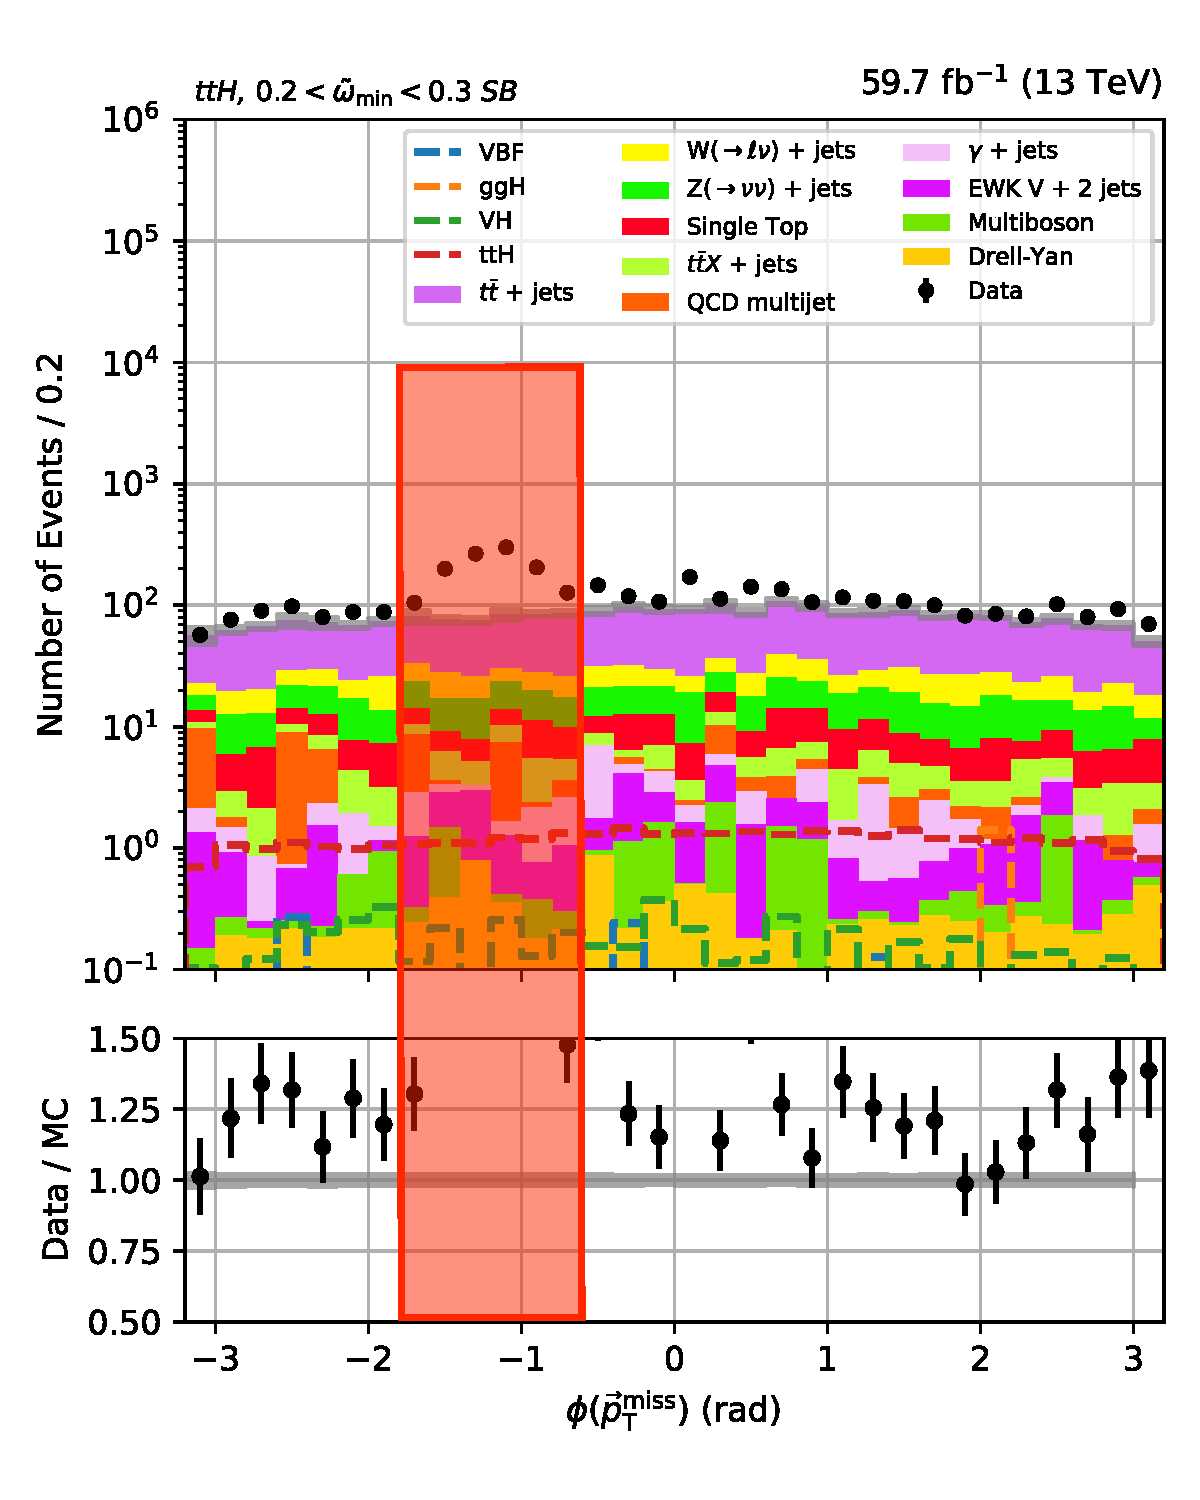
\includegraphics[width=\textwidth]{figures/hem_issue/sideband_4/met_phi/met_phi_ttH_before_annotated.pdf}
        \caption{\ttH category}
    \end{subfigure}
    \hspace{0.05\textwidth}
    \begin{subfigure}[b]{0.34\textwidth}
        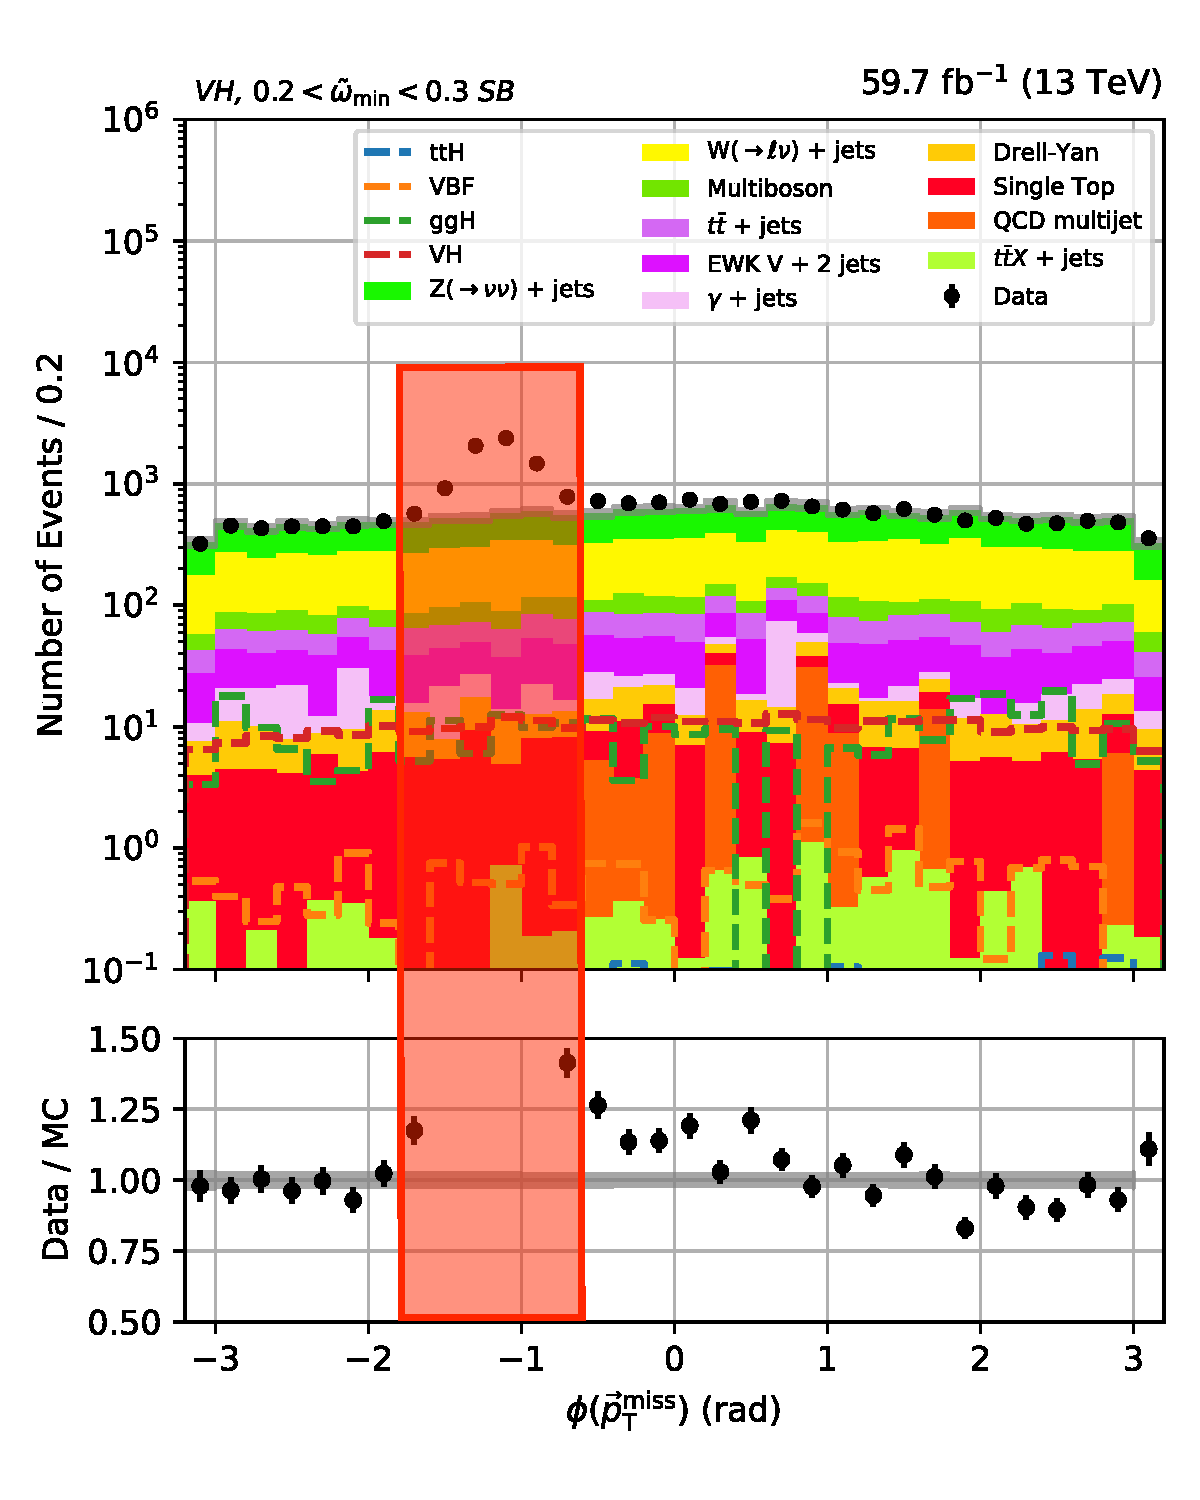
\includegraphics[width=\textwidth]{figures/hem_issue/sideband_4/met_phi/met_phi_VH_before_annotated.pdf}
        \caption{\VH category}
    \end{subfigure}
    \caption[The azimuthal angle of the \ptvecmiss in the \ttH and \VH categories before and after applying the selections designed to mitigate the HEM issue in 2018]{The azimuthal angle of the \ptvecmiss in the \ttH and \VH categories before and after applying the selections designed to mitigate the HEM issue in 2018. The loose \omegaTilde \gls{SB} is used to demonstrate the effect since it kinematically resembles the signal region, and the data--simulation discrepancy can be removed while still blind in said region. A red box encloses the sector that is removed by the selection applied in the signal region and \glspl{SB}.}
    \label{fig:htoinv_hem_issue_met_phi}
\end{figure}

\begin{figure}[htbp]
    \centering
    \begin{subfigure}[b]{0.34\textwidth}
        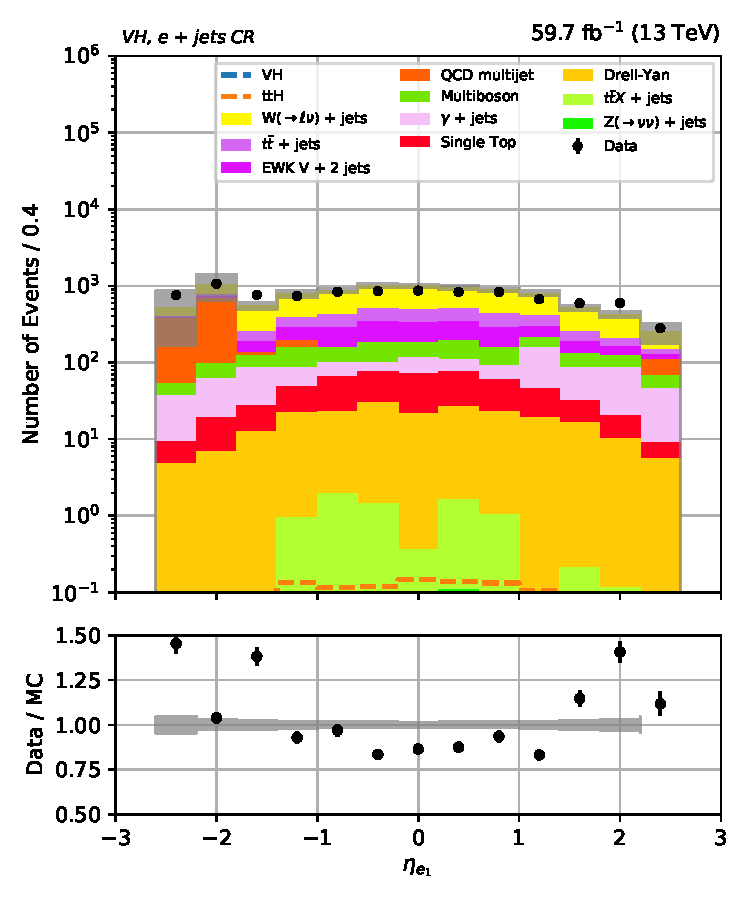
\includegraphics[width=\textwidth]{figures/hem_issue/region_3/leadLepton_eta/leadLepton_eta_VH_before.pdf}
        \caption{$\eta_{\Pe}$ before cut}
    \end{subfigure}
    \hspace{0.05\textwidth}
    \begin{subfigure}[b]{0.34\textwidth}
        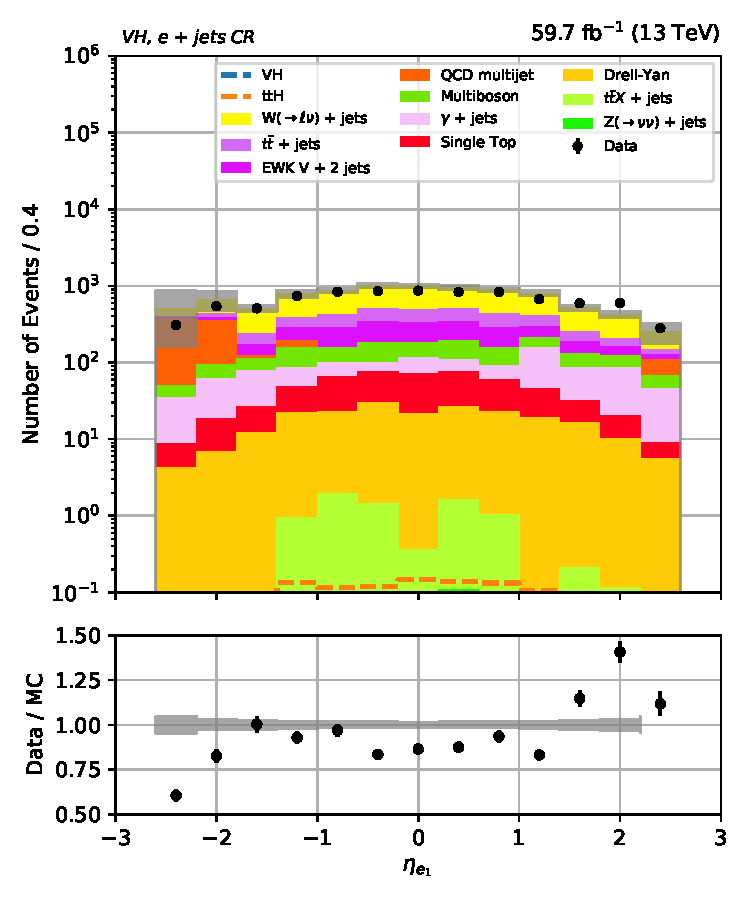
\includegraphics[width=\textwidth]{figures/hem_issue/region_3/leadLepton_eta/leadLepton_eta_VH_after.pdf}
        \caption{$\eta_{\Pe}$ after cut}
    \end{subfigure}
    \caption[The pseudorapidity of the electron in the \VH category of the \singleEleCr \gls{CR} before applying the selection designed to mitigate the HEM issue in 2018]{The pseudorapidity of the electron in the \VH category of the \singleEleCr \gls{CR} before applying the selection designed to mitigate the HEM issue in 2018.}
    \label{fig:htoinv_hem_issue_lepton_eta}
\end{figure}

% Figures from 3rd September, 2020
